\documentclass[man]{apa2}
\usepackage{pslatex}
\usepackage{amssymb}
\usepackage{graphicx}
\usepackage{color}
\usepackage{covington}
\usepackage[usenames,dvipsnames]{xcolor}
\usepackage{booktabs}
\usepackage{setspace}


\title{Understanding the effect of social context on learning: \\ A replication of Xu and Tenenbaum (2007b)}

\twoauthors{Molly L. Lewis}{Michael C. Frank}
\twoaffiliations{Department of Psychology, Stanford University}{Department of Psychology, Stanford University}


\abstract{Does the source of a piece of data---the process by which it is sampled---influence the inferences that we draw from it? Xu and Tenenbaum (2007b) reported a large effect of sampling process on learning: When a category exemplar was presented by a knowledgable teacher, learners generalized more narrowly than when it was presented from an unknowledgable source.  In five experiments, four online and one in-person, we attempted to reproduce this result. Aggregating across our studies, we replicated the original finding of sensitivity to the sampling process, but with a smaller effect size than the original. We discuss these findings in the context of concerns about replicability more generally, as well as the practical relevance of sampling effects in psychological experiments.

~\\

Keywords: word learning, sampling, Bayesian reasoning}

\shorttitle{Replication of Xu and Tenenbaum 2007b}
\rightheader{Replication of Xu and Tenenbaum 2007b}

\acknowledgements{ 

~\\

\noindent Address all correspondence to Molly L. Lewis, Stanford University, Department of Psychology, Jordan Hall, 450 Serra Mall (Bldg. 420), Stanford, CA, 94305. Phone: 650-721-9270. E-mail: \texttt{mll@stanford.edu}
\\
\vspace{10mm}
\noindent Word Count: 5571}

\begin{document}

\maketitle       

\section{Introduction}

Imagine you're hiking up a trail and come to a junction. You see a large branch leaning on the trail, partially blocking one path. Most likely the branch is a bit of random debris that shouldn't affect your decision of which way to hike. But if you know that a friend walked up the trail in front of you just a few minutes before, you might interpret the branch as a signal, intended to point you in the right direction and help you follow her. The intuition underlying this example is that an observation can have a very different meaning depending on its source.

\citeA{xu2007,xu2007word} (XT, below) examine this phenomenon---sensitivity to the sampling process for data---in the context of a particularly difficult inductive problem: concept generalization in word learning. Faced with a novel word and its referent, children must decide between an infinite number of hypotheses about the concept extension of that word. For example, consider a child who hears the word ``apple'' in the context of a single apple on a table. While the referent of that object is clear in the moment of language use (i.e., the particular apple on the table), the broader concept is highly ambiguous: ``apple'' could refer to the category of apples, the category of fruit, that particular kind of apples (e.g., granny smith), green things, or any number of other ad-hoc categories. As a possible solution to this problem, XT proposed a model of word learning as inductive concept learning. In their model, learners observe data as word-object pairs and make inferences about the concept associated with that word from a hypothesis space of all possible meanings. Critically, their model predicts that a learner should generalize more broadly when the exemplar for learning is sampled from the full hypothesis space of meanings ({\it weak sampling}), and should generalize more narrowly when the exemplar is sampled from only those true exemplars of the word ({\it strong sampling}). 

In the study we focus on here, \citeA{xu2007word} asked whether adults and children are sensitive to these differences in sampling process. In their experiment, they altered the strength of the sampling process by manipulating the source of the observed data. Learners in their study were presented with three labeled exemplars from a target category, either provided by a knowledgeable teacher or via the learners'  guesses based on a single labeled exemplar. Importantly, in both conditions, the data that the participants observed was the same: three exemplars from the same subordinate-level category. What differed between conditions was only the sampling process for these exemplars: Since the teacher knew the true concept, the data were presumed to be sampled strongly from the true concept. But in the learner-generated condition, the learner was na\"ive about the true underlying concept and the data were thus presumed to be sampled weakly from the full hypothesis space. 

Participants observed these samples in the context of a display of possible novel category members that showed hierarchical structure such that it could easily be clustered into subordinate, basic level, and superordinate categories. Participants were then tested on how broadly they generalized the concept from the exemplars they observed. The key prediction was that participants in the teacher condition should be more likely to generalize tightly to the subordinate level, while participants in the learner condition should generalize more broadly at the basic level. The empirical data supported this prediction in both adults ($N=14$, $d = 1.49\ [0.01,\ 2.97]$) and children ($N=24$, $d = 1.21\ [.19,\ 2.23]$).

While the focus of XT's study is the problem of word learning faced by children,  the broader theoretical question---how the source of information influences learning---has far-reaching implications for our understanding of human learning more generally.  Every datum is observed in some context, and social aspects of that context can radically change the interpretation of that datum. Evidence for sensitivity to sampling assumptions is thus critical in constraining theories about language learning, concept learning, and the social transmission of information mored generally. The reproducibility of XT's results is therefore of broad import.

Although no experiments that we are aware of have used XT's precise paradigm, a host of related experiments have provided independent evidence for effects of sampling process on learning and inference. For example, \citeA{bonawitz2011double} showed that children interpret evidence about the functionality of a toy differently depending on how the function was demonstrated. In their experiments, children discovered fewer additional functions of a toy when its primary function was demonstrated by a knowledgable teacher, compared to when this demonstration was accidental. This finding suggests that children in the knowledgable teacher condition assumed that there were no additional functions associated with the toy, and thus generalized more narrowly than those in the accidental condition (much like the narrower generalizations found by XT). And a number of other findings with both adults and children provide evidence for some form of ``strong sampling'' in social contexts \cite{navarro2012sampling,frank2012predicting,gweon2010,shafto2012learning}. Thus, we believe that there are good reasons to think that the original XT effect is one example of a broader phenomenon. 

Beyond its theoretical relevance, there are a number of additional reasons to conduct a replication of this study. Although there is now converging evidence for a role of sampling on learning, a related aspect of XT's model---the {\it suspicious coincidence effect}---has faced controversy \cite{xu2007}. XT's model predicts that learners should generalize a label more narrowly when there are more exemplars  of the concept that share subordinate features (e.g., it would be surprising if  ``dax" meant ``dog" given three dalmatian exemplars).  Others, however, have suggested that this finding is highly sensitive to the influence of memory and attention, and  therefore may not be practically relevant for children's word learning \cite{jenkins2015non,spencer2011}. In addition to these critiques, there has been other work challenging the broader modeling approach \cite{marcus2013robust,endress2013bayesian}, as well as work providing converging evidence for this particular finding \cite<e.g.,>{gerken2006decisions,gerken2010}. Thus, better understanding the empirical foundations of XT's model is particularly important in light of this controversy.

XT's study (2007b) is also important to replicate because there are reasons to think that the sampling effect may be sensitive to contextual factors, at both the level of the individual and the task environment. Recent work has revealed large individual variability across participants in the strength of sampling assumptions \cite{navarro2012sampling}, making the strength and consistency of XT's original finding somewhat surprising. At the level of the environment, the original study relies on a social manipulation that is grounded in the interaction between experimenter and participant; such social manipulations tend to have a lower replicability rate \cite{reproProj2015}, perhaps due to difficulties in consistently creating the same context and interaction. More broadly, there is evidence that the social sciences have an overall higher rate of positive findings, relative to the physical sciences \cite{fanelli2010positive}. One explanation of this difference is that  social phenomena are inherently more complex than other phenomena. As a result, theories in the social sciences may be less well specified, and therefore easier to support. Replication provides a method for minimizing this bias.

In addition to these theoretical motivations, there is a practical reason for conducting a replication of this study: the theoretical question at issue in XT's study has consequences for the experimental method in psychology. This is because every datum that is collected in a psychology experiment is collected in some social context. In interpreting data from these experiments, it is therefore important to know how the social context influences participants. XT's study provides a step toward understanding this important issue.

Finally, given the importance of this phenomenon, it is important not only to ask {\it whether} there is an effect of sampling on generalization, but also {\it how big} that effect is. XT's study provides one estimate of the effect size  ($d = 1.49\ [0.01,\ 2.97]$), but a more precise estimate can be obtained by conducting replications and aggregating across these estimates using meta-analytic techniques. By measuring the strength of this effect, rather than merely its presence, we can compare its magnitude to other types of effects, investigate the relative influence of moderators, and build quantitative, rather than qualitative theories.

With these motivations, we conducted a series of five replications of \citeA{xu2007}, four online (Experiments 1, 2,  4 and 5) and one in-person (Experiment 3). The last of these studies (Experiment 5) was a large-sample, exact, pre-registered replication of Experiment 4. Our data are consistent with XT's original report, but suggest an effect substantially smaller in magnitude than the original estimate. In the General Discussion, we reflect on the iterative nature of experimental replications and the challenges related to understanding factors that may lead to successful replications. We conclude by discussing how an understanding of sampling might inform our interpretations of data from psychological experiments in general.

\section{Experiment 1} 
In Experiment 1, we attempted to replicate XT's original design in an online paradigm. 

\subsection{Methods}
\subsubsection{Participants} 
XT's original sample with adults included 14 participants. We recruited 294 adult participants online through Amazon Mechanical Turk. Participants were paid US \$0.25. 

We excluded participants from our analysis who responded ``yes'' to the basic non-match question (see Procedure below; $N=8$) or who did not select subordinate matches in the learning condition ($N = 21$).\footnote{This rate of exclusions in the learner condition is much higher than in the original (0\%). One reason for this difference may have been our mention of ``learning" in the instructions, which could have led some participants to test alternative hypotheses in the training phase.} No participant missed the attention check question. 

In addition, we found that not all participants responded consistently across questions of the same type within a trial, unlike in the original report (for example, a participant might respond ``yes'' to one basic match and ``no'' to another). On the basis of the data in Experiment 1, we decided to adopt two different criteria for categorizing participants' response pattern to deal with this variability: liberal and strict. These exclusions allowed us to more directly compare our data to the original data.  Under our liberal criteria,  we categorized a participant as a basic-level generalizer if they responded ``yes'' to both the subordinate matches and {\it at least one} basic-level match. Under our strict criteria, we categorized a participant as a basic-level generalizer if they responded ``yes'' to both the subordinate matches and {\it both} basic-level matches. Under both criteria, a participant was categorized as a subordinate-level generalizer if they responded ``yes'' to only the subordinate level matches.\footnote{Another possible exclusion strategy is to treat generalization consistency separately for basic and subordinate selections, giving rise to four possible schemes. Across all subsequent experiments, we adopt two of these four schemes as planned analyses (``strict'':consistent basic and subordinate; ``liberal": inconsistent basic, consistent subordinate), but in post-hoc analyses we apply  the other two schemes and  find that this choice does not affect the significance of any of the findings.} We excluded participants from our analysis who could not be categorized under either criterion.  We report the results using the liberal criterion in the Main Text and describe the results using the strict criterion in Appendix A. We adopted this criteria for all five experiments, and in no case does the statistical significance of the results depend on the criterion we used. 

%(consistent basic and subordinate; inconsistent basic and subordinate; consistent basic, inconsistent subordinate; inconsistent basic; consistent subordinate)

Under the liberal criteria, 79 participants could not be categorized as either basic or subordinate-level generalizers, and thus were excluded in order to make our data comparable to the original findings.  This high rate of exclusion may be due in part to the fact that we did not offer an explicit reward for correctly generalizing, unlike in the original (participants received a sticker). With all exclusions, our final sample for Experiment 1 included 195 participants  ($N_{learner} = 101$; $N_{teacher} = 94$).

%In this and subsequent experiments, the majority of these excluded participants did not respond ``yes" to any basic level queries and responded ``no" to at least one subordinate query, under our exclusion scheme.

\subsubsection{Stimuli}
We created four sets of objects similar to the original stimuli (Figure \ref{fig:stims}, left).\footnote{All stimuli, experiments, raw data and analysis code can be found at \url{https://github.com/mllewis/xtSamp}. The analyses can be viewed directly here: \url{http://rpubs.com/mll/xtSampAnalysis}.} There were four basic level category (defined by shape) that included 15 unique objects each. Within each basic level category, there were three subordinate categories, with 5 unique objects each. Subordinate categories were defined by color and pattern. The same novel words were used as the original experiment: ``wug,'' ``tupa,'' ``blicket,'' and ``fep.''
\begin{figure}[t]
 \begin{center} 
 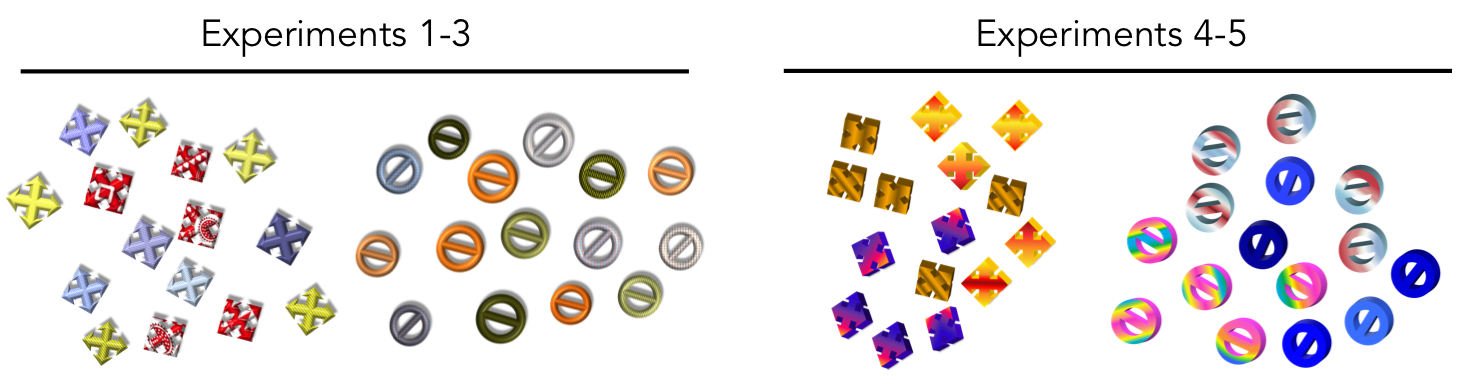
\includegraphics[width=5in]{figures/stims.png} 
 \caption{ \label{fig:stims} Sample stimuli used in Experiments 1--3 (left) and Experiment 4 and 5 (right). The Experiment 4 and 5 stimuli are intended to be maximally similar to the original Xu and Tenenbaum (2007b) stimuli, with lower subordinate-level variability than the stimuli used in Experiments 1--3. All stimuli can be accessed here: \url{https://github.com/mllewis/xtSamp/tree/master/experimentMaterials/stimuli}. } 
 \end{center} 
\end{figure}	
 
\subsubsection{Procedure}
 \begin{figure} [t]
 \begin{center} 
 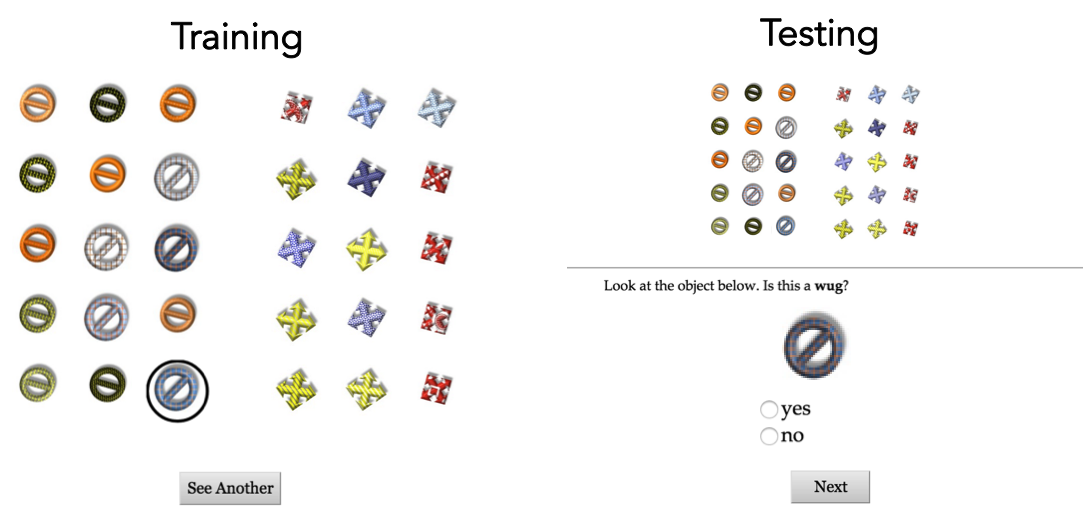
\includegraphics[width=5.5in]{figures/screen.png} 
 \caption{\label{fig:screen} Screen shots of the training (left) and testing (right) phases in Experiment 1. } 
 \end{center} 
\end{figure}


Participants first viewed an instruction page that described the task. In the teacher condition, the instructions read: 
\begin{quote}
In the first part of the experiment, you will see pictures of objects. Some of the objects are called \textit{wugs}. In order for you to learn which objects are \textit{wugs}, I will circle three of them for you. After you learn about the \textit{wugs}, you will be asked questions about them.
\end{quote}
In the learner condition, the instructions were identical except the second sentence above was replaced with: ``In order for you to learn which objects are \textit{wugs} you will try to find two of them. I will tell you whether you are right or wrong.''

Participants then viewed a screen showing all the objects from two basic level categories. Within each basic-level category, the shapes were arranged in a 5 x 3 grid, and the two categories were spatially separated (Figure \ref{fig:screen}). One of the objects in the category on the left was circled. In the teacher condition, the instructions read: ``Find the object that is circled below. That object is a \textit{wug}. When you click on the `See Another' button, I will show you another \textit{wug}.'' The participant was then asked to press a button which caused a circle to appear around one of the exemplars from the same subordinate category as the initially circled object. The participant clicked the button twice in total. 

In the learner condition, the instructions were identical, except the last sentence was replaced with: ``The object circled below is a \textit{wug}. Click on two more \textit{wugs}.'' Participants were then asked to click on two more objects. After each click, a pop-up window appeared with the text ``You're correct! That's a wug.'' This text appeared regardless of the object the participant clicked on (participants who did not select subordinate matches were exclude from the analyses; see Participants above). The display then showed the object with a circle around it to indicate that it had been selected. Critically, in both the teacher and the learner conditions, the nature of the final display was identical: Thirty objects from two basic level categories, with three circled exemplars.

Participants then advanced to the test phase. On the test screen, the objects from the training phase were shown at the top of the page in an identical format to the training phase, but without the exemplars circled. Below these objects was a horizontal line, and a generalization question (Figure \ref{fig:screen}). There were five generalization questions presented sequentially in the same order as in the original report (subordinate match, basic non-match, basic match, subordinate match, basic match). In each test question, the following text appeared, with one of the exemplars below: ``Look at the object below. Is this a wug?'' Participants responded by marking ``yes'' or ``no'' using radio buttons.\footnote{After these questions, we asked several questions related to an additional manipulation irrelevant to the current work.} Finally, we asked an attention check question where participants had to select the label they previously learned from four alternatives.

Object categories and word items were randomized across participants. The order of presentation of the individual objects on the screen was also randomized, as was the placement of the first circle. Sampling condition was manipulated between-participants. This and all subsequent online paradigms can be viewed directly here: \url{https://mllewis.github.io/projects/xtSamp/xtSampindex.html}.

\subsection{Results and Discussion}

 \begin{figure} [t]
 \begin{center} 
 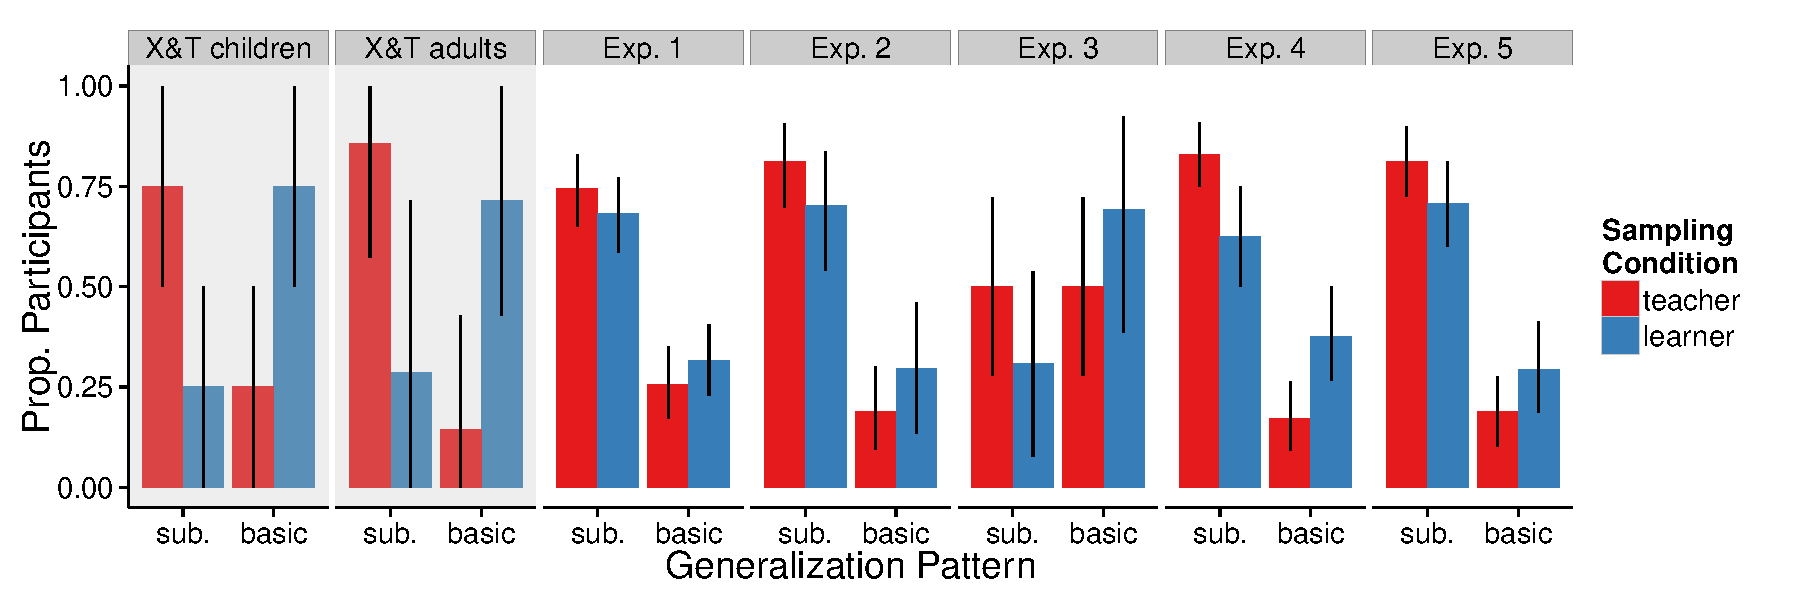
\includegraphics[width=6.2in]{figures/FIG_2.pdf} 
 \caption{\label{fig:bar_plots} Proportion participants generalizing to the subordinate (sub.) or basic level category in the original child ($N = 24$) and adult experiment ($N = 14$), and in our five replication attempts ($N_{1} = 294$; $N_{2} = 150$; $N_{3} = 41$; $N_{4} = 200$, $N_{5} = 500$). Experiments 1, 2, 4 and 5 were conducted online, and Experiment 3 was conducted in-person. Error bars reflect 95\% confidence intervals, calculated via non-parametric bootstrapping. Note that we report the XT data by aggregating across participants, rather than trials (the method in the original report).} 
 \end{center} 
\end{figure}

In the original study, adult participants generalized to the basic level more often in the learner condition compared to the teacher condition ($\chi^2(1) = 2.63$, $p = .11$;\footnote{The original report used a Mann-Whitney test in their analysis, which was statistically reliable. Presumably the choice of the Mann-Whitney test was due to one aspect of the coding scheme for outcomes, which could have yielded a score of 0, 1, or 2 for each participant. Given the more variable responses we received in our initial experiment, we decided against using a code of 1 for intermediate generalization. Instead, we adopted the ``strict'' and ``liberal'' criteria reported above, and selected a categorical data analysis strategy, e.g. $\chi^2$.} $d = 1.49\ [0.01,\ 2.97]$). In current experiment, participants' generalizations were numerically more biased towards basic level generalization in the learner condition, but the difference between sampling conditions was much smaller and was not statistically reliable ($\chi^2(1) = 0.63$, $p = .43$; Figure \ref{fig:bar_plots}). The effect size was also much smaller than the original finding ($d = 0.17\ [-0.17,\ 0.51]$; Figure \ref{fig:effect_sizes}).

\section{Experiment 2}

Given that Experiment 1 did not fully replicate XT's original effect, we attempted to alter our paradigm in Experiment 2 to more closely reflect the original in-person experiments. One critical difference between the in-person and online paradigms was the salience of the experimenter. In the in-person version, the teacher was an actual person interacting with the participant, while in Experiment 1, the reality of the teacher had to be inferred based only on first person text (``I will show you...''). Thus, one reason we might have observed a smaller effect in Experiment 1 is that participants might not have assumed strong sampling in the teacher condition. In Experiment 2, we tried to strengthen this manipulation by introducing a teacher character using a picture.

We also made several other changes to our design. Because many participants in Experiment 1 did not generalize at all (answered ``no'' to all generalization questions), we added questions that queried the original three exemplars that participants learned about. These ``proper name'' trials allowed us to more directly understand these participants' generalization strategy. We also reduced memory demands between the training and testing phases by circling the training exemplars in the testing phase, allowing participants to reflect back on their training data during test.

\subsection{Methods}

\subsubsection{Participants} In Experiment 2, we recruited 150 participants from Amazon Mechanical Turk. Participants were paid US \$0.25 for their participation.

As in Experiment 1, we excluded participants who responded ``yes'' to the basic non-match question ($N=15$) or who did not select subordinate matches in the learner condition ($N = 22$). We also excluded participants who missed any of the attention check questions ($N = 9$).

The criteria for categorizing a participant's generalization strategy were identical to Experiment 1, except for the inclusion of the additional questions. To be categorized as either a subordinate or basic-level generalizer, a participant had to respond ``yes'' to all training items. To be categorized as a basic-level generalizer, a participant had to respond ``yes'' to one of the three basic-level questions under the liberal criteria, and ``yes'' to all three under the strict criteria. Twenty-eight participants were excluded because they could not be categorized as a subordinate or basic-level generalizer.  Our final sample included 90 participants ($N_{learner} = 37$; $N_{teacher} = 53$).


\subsubsection{Stimuli}
The object and word stimuli were identical to Experiment 1.

\subsubsection{Procedure}
The procedure was identical to Experiment 1, with the exception of several key changes described below.

First, we increased the saliency of the experimenter by adding a clipart image of a woman. In the initial instructions, we introduced her by saying, ``Hi, my name is Natalie.'' The image of the teacher was also present in the training and testing phases. These changes were made in both the teacher and learner conditions.

Second, we slightly altered the language of the experimenter to sound more natural. In the learner condition, the instructions in the training phase read: ``Click on two more objects that you think might also be called wugs.'' We also changed the feedback in the training phase to be more conversational, ``Yeah, that's a wug.'' In the testing phase, we added the following text above the training items: ``You identified the objects below as wugs'' (the training exemplars were circled, see below). In the teacher condition, the instructions in the training phase read: ``Find the object that is circled below. That object could be called a wug. When you click on the ``See Another'' button, I will show you another wug.'' In the testing phase, we added ``I showed you these objects were wugs'' above the training items. We also changed the critical question to be ``Could this be called a wug?,'' instead of ``Is this a wug?'' in both conditions. This was done to increase the number of basic-level interpretations of the generalization question. 

Third, we added more generalization questions and randomized their order. Each participant was queried about 10 objects in total: The three training exemplars, two objects from the same subordinate level category as the training exemplars, three basic matches, and two basic non-matches. 

Fourth, we reduced memory demands between the training and testing phases by showing the full set of training items during testing (as in Experiment 1) but leaving the selected exemplars circled. This change ensured that participants remembered which objects had been identified as examples of the target category. 

Finally, we added three additional check questions. We showed participants an object from the target category, as well as two objects from never-seen categories. For each of these objects, we asked ``Did you learn about this kind of object?.'' Participants responded by indicating ``yes'' or ``no'' on a radio button.

\subsection{Results and Discussion}

There was not a reliable effect of sampling on generalization ($\chi^2(1) = 0.89$, $p = .34$; $d = 0.33\ [-0.22,\ 0.88]$). Proportions and effect sizes are shown in Figures \ref{fig:bar_plots} and \ref{fig:effect_sizes}, respectively.

\section{Experiment 3}

Despite increasing the saliency of the teacher, we did not replicate the original effect in Experiment 2. We remained concerned that the teacher was less salient in our version, however, relative to the original. To address this possibility, we next conducted an exact replication of the original study in the laboratory with a real experimenter.

\subsection{Methods}

\subsubsection{Participants} 

In Experiment 3, we recruited 41 undergraduate participants. Participants received either course credit or payment (US \$5.00) for their participation. 

We excluded one participant who did not select subordinate-level matches in the training phase. We also excluded nine participants because they could not be categorized as a subordinate or basic-level generalizer. Our final sample included 31 participants ($N_{learner} = 13$; $N_{teacher} = 18$),

\subsubsection{Stimuli}

The object and word stimuli were identical to Experiments 1 and 2. 

\subsubsection{Procedure}

The procedure in Experiment 3 closely followed the original. The experimenter presented 15 objects from two basic-level categories on two pieces of paper. On each paper, the objects were spatially unstructured. As in the original, the experimenter asked five generalization questions (see Experiment 1) and each participant completed two trials such that they were trained and tested on two different categories. Participants were incentivized in the training phase with a sticker. The exact script used by the experimenter is given in Appendix B. 

\subsection{Results and Discussion}

There was not a reliable effect of sampling condition on generalization ($\chi^2(1) = 0.49$, $p = .48$; $d = 0.45\ [-0.38,\ 1.28]$). One notable difference in this experiment, however, was the rate of generalizations to the basic level: In Experiment 3, there were overall more basic level generalizations compared to the online versions. We return to this difference in the General Discussion.

\section{Experiment 4}
Given that the observed effect in Experiment 3 was only slightly larger than the two previous studies, we inferred that the smaller effect sizes we observed were not due primarily to the decreased saliency of the experimenter. In the next replication, we explored another possible difference between our experiments and the original: the object stimuli. While similar to the original, our objects had slightly more variability within each subordinate level than the original (e.g., in Figure 1, the red subordinate category on the left has a variable pattern). This increased variability may have led participants to be less likely to generalize to the basic level. Thus, in Experiment 4, we conducted an online replication using the same procedure as Experiment 2, but with less variable objects at the subordinate-level. 

\subsection{Methods}

\subsubsection{Participants}  

We recruited 200 participants from Amazon Mechanical Turk. Participants were paid US \$0.30 for their participation.

As in the previous experiments, we excluded participants who responded ``yes'' to the basic non-match question ($N=17$) or who did not select subordinate matches in the learning condition ($N = 27$). We also excluded participants who missed an attention check question ($N = 10$). An additional twenty-one participants were excluded from our analyses because they could not be categorized as a subordinate or basic-level generalizer.  Our final sample included 140 participants ($N_{learner} = 64$; $N_{teacher} = 76$). 

\subsubsection{Stimuli}

The objects contained less subordinate-level variability than that used in Experiment 1--3, and were highly similar to the original (Figure \ref{fig:stims}, right).

\subsubsection{Procedure}

The procedure was identical to Experiment 2.

\subsection{Results and Discussion}


There was a reliable effect of sampling on generalization: Participants in the teacher condition were more likely to generalize to the subordinate category, while participants in the learner condition were more likely to generalize to the basic-level ($\chi^2(1) = 6.42$, $p = .01$; $d = 0.59\ [.15,\ 1.03]$). This dataset thus replicates the pattern seen in the original XT report, though with a much smaller effect size.

\section{Experiment 5}

In our final experiment, we repeated Experiment 4 with a pre-registered sample size based on the effect size estimated from Experiments 1--4 and the XT adult experiment. 

\subsection{Methods}

\subsubsection{Participants}  

To determine the sample size for Experiment 5, we conducted a power analysis based on the effect size estimated from our four replications attempts and the original adult experiment. Using this  effect size, a sample size of 355 was required to  achieve 95\% power on the chi-squared test. Given approximately 35\% data loss in the previous online experiments, we decided on a sample size of 500 participants. We pre-registered our sample size on Open Science Framework (\url{https://osf.io/5xg96/wiki/home/}). Due to an initial error in power calculations, the final sample was collected in two separate groups. As in Experiment 4, participants were recruited on Amazon Mechanical Turk and  paid US \$0.30 for their participation. 

We used the same exclusion criteria as in Experiment 4. We excluded participants who responded ``yes'' to the basic non-match question ($N=40$) or who did not select subordinate matches in the learning condition ($N = 63$). We also excluded participants who missed an attention check question ($N = 21$). An additional sixty-one participants were excluded from our analyses because they could not be categorized as a subordinate or basic-level generalizer. Our final sample included 347 participants ($N_{learner} = 154$; $N_{teacher} = 193$). 

\subsubsection{Stimuli}

The stimuli were identical to Experiment 4.

\subsubsection{Procedure}

The procedure was identical to Experiment 4.

\subsection{Results and Discussion}

As in Experiment 4, there was a reliable effect of sampling on generalization: Participants in the teacher condition were more likely to generalize to the subordinate category, while participants in the learner condition were more likely to generalize to the basic-level ($\chi^2(1) = 24.49$, $p <.001$; $d = 0.71\ [.43,\ .99]$).

\section{Meta-analytic Synthesis}

\begin{figure}[t]
  \centering
  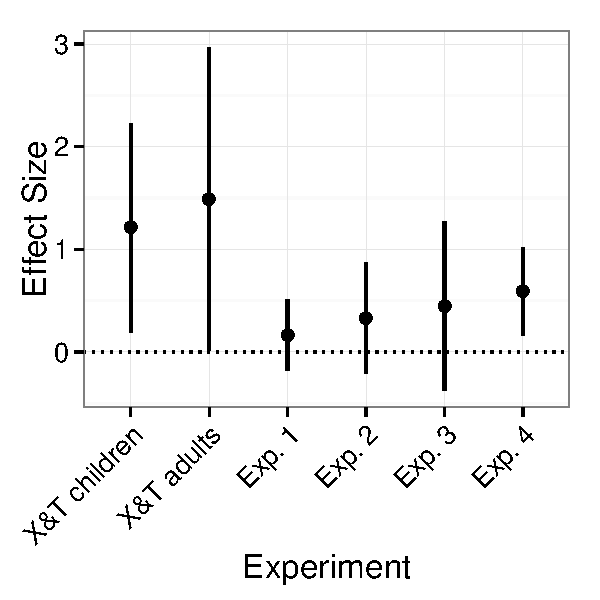
\includegraphics[width=6in]{figures/FIG_3.pdf} 
  \caption{\label{fig:effect_sizes} Effect sizes for XT's original experiment with children and adults, and our five replication attempts. Effect size estimates are calculated  by transforming log odds ratio into Cohen's $d$ (S\'{a}nchez-Meca, Mar\'{i}n-Mart\'{i}nez, \& Chac\'{o}n-Moscoso, 2003; Del Re, 2013). The red diamond indicates the estimate based on a random effect model of all seven studies. Error bars are 95\% confidence intervals.} 
\end{figure}

To obtain the best estimate of the underlying effect size, we used meta-analytic methods to aggregate across estimates from each study. We defined a random effects model based on the estimates from all seven studies \cite{Viechtbauer2010}. The random effect model treats each effect size estimate as an estimate of an underlying population effect size, and weights it by the precision of the estimate (sample size). We elected to include XT's developmental data in the meta-analysis in order to give maximal weight to the larger effects that they observed, which could have been due to some aspect of their method that we did not reproduce.

Across all seven studies, the estimated effect size was .53 ($[.28,\ .78]$; Figure \ref{fig:effect_sizes}). This estimate was only slightly reduced when the original experiment with children was excluded ($d = .50\ [.24,\ .75]$). Thus, we replicate the original effect of sampling on generalization (which was $d = 1.49\ [0.01,\ 2.97]$), but our best guess is that the effect size is approximately one-third as large as estimates reported in the original.

\section{General Discussion}

We attempted to replicate a theoretically-important effect first reported by Xu and Tenenbaum (2007b): sensitivity to sampling process in inductive generalization. Across five replication attempts, we found a statistically significant effect in the same direction as the result in two; the other three attempts found results that were numerically congruent though weaker. To obtain an estimate of the overall effect size, we used meta-analytic methods to aggregate across estimates from each study. We found strong evidence of a real effect, albeit one with an estimated size approximately one-third the magnitude of the original. 

%This effect is consistent with a set of broader findings related to the role of sampling in social contexts. 

\subsection{Reflections on replication}

Although we attempted to reproduce XT's original paradigm as closely as possible, there were a number of differences both across studies and within each individual study that differed. Some of our studies were online (1, 2, 4, and 5), while one was in person; some of our studies used less variable stimuli (4, 5) while others used stimuli with slightly more variability (1, 2, 3); some of our online studies pictured the teacher (2, 4, 5), while one did not (1). Examining our estimated effect sizes, it is tempting to try and synthesize these variations with the different magnitudes of our estimated effects and assume that each of these factors is a moderator of effect size. Such a conclusion is unwarranted by our data however. 

It is of course \emph{possible} that the .16 effect size difference between Experiments 1 and 2 was \emph{caused} by the addition of the teacher's face and the text modifications that we made. But nearly the exact same difference in effect size (.16) is observed between Experiments 4 and 5, where there is no difference whatsoever. 
%More generally, it is virtually impossible to gain empirical traction on moderators whose effects are in the range of $d = .1$. Measuring such effects with appropriate statistical power requires thousands of participants, and will not be a fruitful exercise in a case where many such tiny moderators could exist. 
There may also be larger moderators that were responsible for the difference between the large effect observed by XT and the smaller effects we observed. Social paradigms like XT's likely are sensitive to the details of the social interaction between teacher and participant, the incentive structure in the task, the visual variability of the stimuli, and the spatial layout of the stimuli, to name a few factors. Indeed, the larger degree of basic-level generalization that both we and XT observed in the lab (compared with our online samples) may suggest that online participants felt compelled to be overall more conservative in their generalizations. They may have placed greater value on ``getting it exactly right,'' and therefore been less likely to generalize more broadly to the basic level under uncertainty. 

There is also a priori reason to believe that object variability might influence the effect size. High variability at the subordinate level results in subordinate-level categories that are less distinctive from each other, and the theory of generalization implemented by XT predicts a weaker effect of sampling for less distinctive subclasses \cite{tenenbaum2001generalization}. Indeed, there is some  preliminary evidence for this difference in a meta-analysis that  only includes experiments that used  the less-variable stimuli (XT, Exp. 4 and 5): With this subsample of experiments, the overall effect size estimate was somewhat larger ($d = .72\ [.50,\ .95]$), relative to the estimate with all experiments ($d = .50\ [.24,\ .75]$). 

However, while directly testing for these moderators is possible in principle, the small size of these effects make them difficult and expensive to identify. For example, one could  test whether an in-person version of the experiment has a larger effect size than an online design. This could be done by comparing the effect sizes in Experiments 1 and 2 to Experiment 3. Or alternatively, an additional experiment could be conducted with the improved stimuli in the lab and compared to Experiments 4 and 5.  It is difficult to know what the appropriate power analysis is for a test of this hypothesis, because the analysis depends on many decisions---which experiments to compare to, what effect size estimate to use, and how to structure the comparison. For example, should a planned experiment conduct a comparison with previous studies, or directly manipulate the variable of interest? We conducted a number of these sorts of power analyses under different sets of assumptions; most required collecting data from upwards of 100 participants in the lab. Given this variability, a conservatively-powered experiment would likely require substantial effort, and may even then not provide conclusive evidence. There may be cases where testing for these moderators is indeed theoretically important. But, in other cases where the effects of the moderators are thought to be small, conducting additional experiments to test for them may not be a fruitful exercise.

%Our studies did not allow us to identify such moderators of the experimental manipulation, however.

One final possibility is that there are  \emph{no} moderators that explain the difference between XT�s original result and ours; that is, the observed difference is due instead to chance variation. Most effect sizes in psychology are in the range we estimated for XT's effect \cite{richard2003}, and often the first measurement of an effect is larger than a replicated effect size, even if the replication is successful \cite{reproProj2015}. Recall that XT's original theory made no prediction about the size of the effect, and that $d=.5$ is generally classified as a medium effect \cite{cohen1992}.

In the context of this discussion, we believe that the most appropriate conclusion is that our data support an effect of statistical sampling process on generalization, and that the magnitude for this particular paradigm is likely to be similar to our meta-analytic estimate. We conclude by considering a practical implication of XT's finding: the role of sampling in psychological experiments.

\subsection{Sensitivity to sampling in experimental contexts}

XT's finding suggests that the social context of information influences generalization in a word learning task. But, if this effect holds for human learning more generally, this finding has important consequences for the interpretation of data collected in psychological experiments: the presence of an experimenter---either explicit or implied---may influence how participants interpret and respond to experimental stimuli.

Experimental data are often consistent with at least two accounts---an account that relies on reasoning about the intention of the experimenter, and an account that relies on context-independent reasoning. Consider two examples. A well-known phenomenon in word learning is that children are biased to select a novel object for a novel word, given the presence of both a familiar and novel object \cite<often referred to as {\it mutual exclusivity} in the literature;>{markman1988}. On the one hand, this result could be due to a context-independent bias to assume that lexicons are structured with one word mapping to one concept, and one concept mapping to one word. But another possibility relies on reasoning about the intentions of the experimenter \cite<Why would the experimenter use a strange word to refer to the familiar object if she meant the familiar one?;>{clark1987principle, clark1988logic}. Both of these accounts make similar predictions, and are therefore difficult to disentangle empirically.

Another example of this interpretative ambiguity is the classic \citeA{heider1944} study. In this task, participants viewed a short movie showing several geometric shapes moving in a way that appeared to be contingent. Nearly all participants spontaneously interpreted the video as depicting animate beings, rather than as simple shapes moving around. As in the case of mutual exclusivity, there are at least two ways to interpret this result. One possibility is that participants rely on low-level features of the scene to infer animacy (e.g., contingency), but another possibility is that participants infer the intention of the \emph{experimenter} to be the creation of the videos in order to depict an animate scenario.

These two cases---mutual exclusivity and animacy projection---illustrate a pervasive theoretical issue in experimental psychology. Experimental data are almost always consistent with both social and asocial accounts. There is no simple solution to this empirical challenge: it is impossible to eliminate social context from experimental paradigms, because experiments are social interactions between participant and experimenter. Our best bet is to try and understand the influence of social context on learning. On this view, then, XT's paradigm provides one robust datapoint that informs this project.

In sum, the data presented here shed light on a theoretically important question: How does the source of data influence learning?   XT's original results have been both influential and controversial. Through a series of  detailed replications, our data substantiate the original sampling effect, but also provide an estimate of its magnitude. In light of the  broader interest in replicability and reproducibility across psychology \cite{reproProj2015},  our studies can be thought of as a case study of how the scientific process can productively proceed on the basis of a single positive finding. Through cross-lab replications and iterative experiments, psychologists can aggregate across studies---each individually noisy---to obtain better estimates of true, underlying psychological phenomena.


\section{Appendix A}

Table \ref{tab:strictResults} give results of all five experiments using the strict categorization criteria.

\begin{table}[h]
\centering
\begin{tabular}{rrrrr}
 \hline
 & N excluded & $\chi^2$ & $p$ & $d$ \\ 
 \hline
Exp. 1 & 94 & 0.08 & .78 & $0.09\ [-0.30,\ 0.48]$\\ 
Exp. 2 & 36 & 0.07 & .79 & $0.19\ [-0.46,\ 0.85]$ \\ 
Exp. 3 & 14 & 0.63 & .43 & $0.53\ [-0.35,\ 1.41]$ \\ 
Exp. 4 & 31 & 4.13 & .04 & $0.54\ [0.06,\ 1.02]$\\ 
Exp. 5 & 92 & 17.20 &  .00 & $0.70\ [.36,\ 1.04]$\\ 
 \hline
\end{tabular}
\caption{\label{tab:strictResults} Results of all five experiments using the strict categorization criteria, described in Experiment 1. ``N excluded'' refers to the number of participants excluded from analyses because they could not be categorized as either basic or subordinate-level generalizers. All $\chi^2$ tests have 1 degree of freedom. The overall effect size is  $d = 0.51\ [.22,\ 0.79]$, using the  meta-analytic model described in the Main Text.}
\end{table}

%\section{Appendix B}

%Table \ref{tab:liberalexclusions} summarizes the generalization strategies of participants who were excluded from the analysis under the liberal criteria.
%\begin{table}[h]
%\centering
%\begin{tabular}{rrrr}
% \hline
%  & Condition & No basic/inconsistent sub. & Some basic/inconsistent sub. \\ 
%  \hline
%   Exp. 1  &  teacher      &               .98       &           .02\\
 % Exp.  1 &   learner        &           .93         &        .07\\
%   Exp.  2 &    teacher     &             .96        &       .05\\
%   Exp. 2 &    learner    &               1.00        &                    .00\\
%   Exp. 3  &  teacher   &                1.00    &                        .00\\
%   Exp.  3 &  learner    &               1.00   &                         .00\\
%    Exp.   4 & teacher   &                 .94   &                 .06\\
%    Exp. 4 &     learner    &           1.00      &                      .00\\
%    Exp. 5 &     teacher   &                .95    &              .05\\
%    Exp. 5   &  learner     &             .83      &          .17\\
% \hline
%\end{tabular}
%\caption{\label{tab:liberalexclusions} Under the liberal criteria, excluded participants fell broadly into two categories: (1) those who responded ``no" to all basic level queries and  inconsistently to the subordinate queries, and  (2)  those who responded ``yes" to at least one basic query, but responded inconsistently to the subordinate level queries. Presented here are the proportion of excluded participants in each experiment and condition for each broad exclusion category. 
%}
%\end{table}


\section{Appendix B}
Below is the script used by the experimenter in Experiment 3. ``[word]'' denotes a randomly selected novel label. Different labels and objects were used in Trial 1 and Trial 2. 

\vspace{5mm}

{\it Thank you for participating in this study. We're going to play a game that was initially designed for preschoolers, so it may seem a little silly, but just play along. Are you ready to begin?}
\vspace{2.5mm}

\noindent \underline{Training} \\
	Teacher Condition: {\it See this? It's a [word]. See this one? It's a [word]. See this one? It's a [word]. Thank you for paying attention. Would you like to choose a sticker? }
\\
Learner Condition: {\it See this? It's a [word]. Can you point to two other [word]s? If you get both of them right you get a sticker! You're correct! You're correct! Would you like to choose a sticker? }
\vspace{2.5mm}
 
\noindent \underline{Testing} \\
{\it Alright, now I'm going to ask you some questions about [word]s. Are you ready?} \\
$\langle$point to subordinate$\rangle$ {\it Is this a [word]?} \\
$\langle$point to basic non-match $\rangle$ {\it Is this a [word]?} \\
$\langle$point to basic match$\rangle$ {\it Is this a [word]?}\\
$\langle$point to subordinate$\rangle$ {\it Is this a [word]?} \\
$\langle$point to basic match$\rangle$ {\it Is this a [word]?} \\
 
{\it Alright, now I'm going to show you some new shapes. Are you ready?}\\

\vspace{2.5mm}
\noindent $\langle$repeat Training and Testing for Trial 2$\rangle$ \\
\noindent {\it All done! Thank you for participating!}

\nocite{re2013}
\nocite{sanchez2003effect}

\section{Acknowledgments}

We gratefully acknowledge Josh Tenenbaum and Fei Xu for helpful comments and discussion. We also thank Marlene Ade for her help with data collection and Ann Nordmeyer for helpful feedback on the manuscript. 

\bibliographystyle{apacite2}
\bibliography{biblibrary}

\newpage
\theappendix 
\end{document}
